\documentclass[DIV=33,landscape,paper=a3,12pt]{scrartcl}
\usepackage{dingbat}
\usepackage[hidelinks]{cleveref}
%\hypersetup{
%pdftitle={Pentagame Regulae Rules Regeln Regles},
%pdfsubject={Pentagame Rules in Many Languages},
%pdfauthor={Jan Suchanek et al.},
%pdfkeywords={Pentagame board game rules explained latin english german deutsch latine francais russian chinese spanish espaniol}
%}

\usepackage[symbol]{footmisc}
\renewcommand*{\thefootnote}{\fnsymbol{footnote}}
 \usepackage{ragged2e} 
\usepackage{enumitem}

\usepackage[dvipsnames]{xcolor}
\usepackage{tikzpeople}

\usepackage{framed}
\usepackage{polyglossia}
\usepackage{xeCJK}
\providecommand{\chapterformat}{}
\setmainlanguage{english}
\setotherlanguages{french,ngerman,latin,bahasai,russian,greek,spanish,georgian,swedish,polish}

\DeclareTextCommandDefault{\cyrdash}{\hbox to.8em{---}~}

\makeatletter
\newcommand\footnoteref[1]{\protected@xdef\@thefnmark{\ref{#1}}\@footnotemark}
\makeatother

\setmainfont{FreeSerif}
\setsansfont{FreeSans}
\newCJKfontfamily{\tradChinesefont}{AR PL UKai HK}[BoldFont=Noto Sans CJK TC Bold]

\usepackage{setspace}
\usepackage{multicol}
\usepackage{titlesec}
\usepackage{microtype}
% \usepackage{CJKutf8}
\usepackage{pgfpages,tikz,lipsum}
\usetikzlibrary{calc}
\usetikzlibrary{shapes.multipart}
\usetikzlibrary{arrows}
\usetikzlibrary{shapes.misc}
\usetikzlibrary{decorations.text}
\usetikzlibrary{automata, positioning}
\usetikzlibrary{hobby}
\usetikzlibrary{decorations.markings}
\usetikzlibrary{patterns}

%\usepackage{CJK}
\usepackage{tikz}
\raggedbottom
\raggedcolumns
\clubpenalty = 10000
\widowpenalty = 10000
\displaywidowpenalty = 10000

\newcommand{\noun}[1]{\textsc{#1}}


\newcounter{oldpage}


\makeatletter
\renewcommand\paragraph{%
\@startsection{paragraph}{4}%
{\z@}{1ex\@plus 1ex \@minus .2ex}%
{0.2ex \@plus .2ex}%
  {\sffamily\normalsize\bfseries}%
 }
 \makeatother

%%% Document specific commands

\newcommand{\myskip}{\smallskip}

\newcommand{\headline}{{\LARGE{}Pentagame}}
\newcommand{\tocent}{}
\newcommand{\translator}{}

\newcommand{\general}{}
\newcommand{\choosext}{}
\newcommand{\choosex}{}
\newcommand{\setupt}{}
\newcommand{\setup}{}
\newcommand{\objectivet}{}
\newcommand{\objective}{}
\newcommand{\rulest}{}
\newcommand{\rules}{}
\newcommand{\website}{\textsf{\textbf{pentagame.org}}}
\newcommand{\layout}{
\begin{centering}

{\sffamily\LARGE{\textbf\headline}}
\addcontentsline{toc}{section}{\tocent}

\end{centering}

\bigskip

\hrulefill


\begin{multicols}{2}

%\noindent\hrulefill
\general
\paragraph*{\choosext}
\choosex
\paragraph*{\setupt}
\setup
\paragraph*{\objectivet}
\objective


\medskip
\parbox{\columnwidth}{
\paragraph*{\rulest}
\rules
}

\end{multicols}}

\setlength{\parskip}{0ex}
\setlength{\parindent}{0cm}


\title{
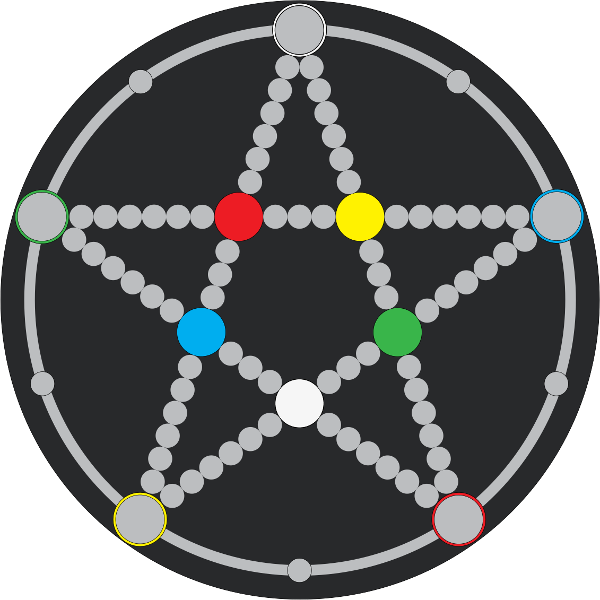
\includegraphics[width=0.5\textwidth]{Pentagame_board_2018.png}\\
Penta$\cdot$game}
%\subtitle{by Jan Suchanek}
\author{ \href{mailto:jan@pentagame.org}{\makeatletter jan@pentagame.org\makeatother} }
\date{}

%% Actual Document. Calling the content first, then printing the same layout.

\begin{document}

%\maketitle

\begin{framed}
\centering
{\sffamily{\Huge{\textbf{How to play Pentagame}}}}
\end{framed}

\begin{multicols}{5}

\setlength{\columnseprule}{0.4pt}

\centering

    \titlespacing*{\section}
{0pt}{1ex plus 1ex minus .2ex}{-2.3ex plus .2ex}

\newcommand{\skipper}[1]{\medskip\section{#1}~\\\smallskip }

\newcommand{\skipperstar}[1]{\medskip\section*{#1}~\\\smallskip }


\def \n {5} \def \radius {0.5\columnwidth} \def \raz {1.2cm}    \def \radiusz {0.7\columnwidth}

\usetikzlibrary{shapes}

\tikzset{state/.style={circle, draw, inner sep=0.25cm, opacity=1, fill=black, minimum size=0.2pt}}

\tikzset{statez/.style={diamond,draw, thick, inner sep=0.1cm, opacity=1, fill=black, minimum size=0.2pt}}

\tikzset{statezz/.style={regular polygon,regular polygon sides=3,draw, thick, inner sep=0.08cm, opacity=1, fill=black, minimum size=0.2pt}}
\tikzset{staten/.style={diamond, thick, inner sep=0.1cm,  minimum size=0.2pt}}

\tikzset{stateb/.style={regular polygon, regular polygon sides=7, thick, inner sep=0.1cm, opacity=1, fill=black, minimum size=0.2pt}}

\tikzset{node distance=1mm}

\tikzset{cross/.style={cross out, draw=black, minimum size=2*(#1-\pgflinewidth), inner sep=2pt, outer sep=2pt},
    cross/.default={1pt}}  

\newcommand{\boardy}{
    % lines
    \foreach \s in {1,...,\n} { 
    \draw[dashed, >=latex] ({360/\n * (\s - 1)}:\radius)      arc ({360/\n * (\s - 1)}:{360/\n * (\s)}:\radius);   
    \draw[dashed,gray,line width=3pt,line cap=round, dash pattern=on 1pt off 8.5\pgflinewidth, >=latex] ({360/\n * (\s - 1)}:\radius)      arc ({360/\n * (\s - 1)}:{360/\n * (\s)}:\radius);   
    \draw[dashed,black!50, line width=3pt,line cap=round, dash pattern=on 1pt off 1.83\pgflinewidth, >=latex] ({360/\n * (\s - 2)+90}:\radius)      -- ({360/\n * (\s)+90}:\radius); 
    } 
    % nodes
    \node[state, fill=white] (1) at ({360/\n * (1 - 1)+90}:\radius) {};  
    \node[state, fill=white] (1a) at ({360/\n * (1 - 1)+90}:-\radius/2.618) {};     
    \node[state, fill=Cerulean] (2) at ({360/\n * (2 - 1)+90}:\radius){};  
    \node[state, fill=Cerulean] (2a) at ({360/\n * (2 - 1)+90}:-\radius/2.618) {};     
    \node[state, fill=WildStrawberry] (3) at ({360/\n * (3 - 1)+90}:\radius) {};  
    \node[state, fill=WildStrawberry] (3a) at ({360/\n * (3 - 1)+90}:-\radius/2.618) {}; 
    \node[state, fill=Goldenrod] (4) at ({360/\n * (4 - 1)+90}:\radius) {};     
    \node[state, fill=Goldenrod] (4a) at ({360/\n * (4 - 1)+90}:-\radius/2.618) {};    
    \node[state, fill=LimeGreen] (5) at ({360/\n * (5 - 1)+90}:\radius) {};       
    \node[state, fill=LimeGreen] (5a) at ({360/\n * (5 - 1)+90}:-\radius/2.618) {};     
}
    


    

  



  %  \centering
    

    
    
    
    \skipper{Choose pieces}

\begin{tikzpicture}
        \node[alice, minimum size=1cm] at (-1,1.618) (alice) {};
        \node[statez, fill=white] at (1,1.618) {};
        \node[statez, fill=Cerulean] at (2,1.618) {};
        \node[statez, fill=WildStrawberry] at (3,1.618) {};
        \node[statez, fill=Goldenrod] at (4,1.618) {};
        \node[statez, fill=LimeGreen] at (5,1.618) {};
        \node[bob, minimum size=1cm] at (-1,0) (bob) {};
        \node[statezz, fill=white] at (1,0) {};
        \node[statezz, fill=Cerulean] at (2,0) {};
        \node[statezz, fill=WildStrawberry] at (3,0) {};
        \node[statezz, fill=Goldenrod] at (4,0) {};
        \node[statezz, fill=LimeGreen] at (5,0) {};

\end{tikzpicture}
        
    Everyone has pieces of one \textbf{shape.}
    Pentagame is for 2, 3 or 4 players.
    
\hrulefill    
    
\skipper{Setup your pieces} 
    
\begin{tikzpicture}[scale=0.65]

    \scriptsize
    
    \begin{scope}[xscale=-1]

    \boardy
    
    \node  (1z) at ({360/\n * (1 - 1)+90}:\radiusz) {};  
    \node  (2z) at ({360/\n * (2 - 1)+90}:\radiusz){};  
    \node  (3z) at ({360/\n * (3 - 1)+90}:\radiusz) {};  
    \node  (4z) at ({360/\n * (4 - 1)+90}:\radiusz) {};     
    \node  (5z) at ({360/\n * (5 - 1)+90}:\radiusz) {};       
    
    \node[statez, fill=white] (1t) at (1) {};  
    \node (01) at (1z) {};  
    \node[statez,left=of 01,fill=white] (01z)  {};  
    \node[statezz,right=of 01,fill=white] (01zz)  {};  
    
    \node[statez, fill=Cerulean] (2t) at (2){};   
    \node (02) at (2z){};   
     
    \node[statez,above left=of 02,fill=Cerulean] (02z)  {};  
    \node[statezz,below=of 02,fill=Cerulean] (02zz)  {};  
      
    \node[statez, fill=WildStrawberry] (3t) at (3) {};  
    \node (03) at (3z) {};      
    
    \node[statez,below left=of 03,fill=WildStrawberry] (03z)  {};  
    \node[statezz,right=of 03,fill=WildStrawberry] (03zz)  {};  
    
    \node[statez, fill=Goldenrod] (4t) at (4) {}; 
    \node (04) at (4z) {}; 
     
    \node[statez,above left=of 04,fill=Goldenrod] (04z)  {};  
    \node[statezz,below right=of 04,fill=Goldenrod] (04zz)  {};      
       
    \node[statez, fill=LimeGreen] (5t) at (5) {};   
    \node (05) at (5z) {}; 
     
    \node[statez,below=of 05,fill=LimeGreen] (05z)  {};  
    \node[statezz,above right=of 05,fill=LimeGreen] (05zz)  {};      
    
    \draw[>=triangle 45, line width=1.5pt, ->] (01) -- (1) ;
    \draw[>=triangle 45, line width=1.5pt, ->] (02) -- (2) ;
    \draw[>=triangle 45, line width=1.5pt, ->] (03) -- (3) ;
    \draw[>=triangle 45, line width=1.5pt, ->] (04) -- (4) ;
    \draw[>=triangle 45, line width=1.5pt, ->] (05) -- (5) ;    
    \end{scope}
\end{tikzpicture}
    
    
    All pieces start at the rim, on the corner of their colour.

    
  
\hrulefill

\skipper{Setup blocks}

\newsavebox{\mybox}
\sbox{\mybox}{%    
    \begin{tikzpicture}[node distance=-3pt]
        \node (nil) {};
        \node[statez,fill=none,scale=0.7,left=of nil] (z) {} ;
        \node[statezz, right=of nil, fill=none,scale=0.7] (zz) {};
    \end{tikzpicture}
}

\begin{tikzpicture}[scale=0.65]

    \scriptsize
    \begin{scope}[xscale=-1]

    \boardy

    
    %\node[statez, fill=white] (1t) at (1) {};  
     
    \node (1t) at (1) {\usebox{\mybox}};  
    \node  (2t) at (2){\usebox{\mybox}};   
    \node  (3t) at (3){\usebox{\mybox}};   
    \node  (4t) at (4){\usebox{\mybox}};       
    \node  (5t) at (5){\usebox{\mybox}};   
     
    \node[stateb, fill=black] (1b) at (1a) {}; 
     
 %   \node  (2t) at (2){\usebox{\mybox}};   
     
    \node[stateb, fill=black] (2b) at (2a) {}; 
      
 %   \node[statez, fill=WildStrawberry] (3t) at (3) {};      
    
    \node[stateb, fill=black] (3a) at (3a) {}; 
    
  %  \node[statez, fill=Goldenrod] (4t) at (4) {};     
     
    \node[stateb, fill=black] (4a) at (4a) {}; 

%    \node[statez, fill=LimeGreen] (5t) at (5) {};           
     
    \node[stateb, fill=black] (5b) at (5a) {};     
    
    \end{scope}
\end{tikzpicture}
   
    Put \textbf{black blocks on the crossings.}
    
    They are neutral.
    
    \begin{tikzpicture}[scale=0.65]
        \node[stateb, fill=gray] (g1) at (-2,-6) {}; 
        \node[stateb, fill=gray] (g1) at (-1,-6) {}; 
        \node[stateb, fill=gray] (g1) at (0,-6) {}; 
        \node[stateb, fill=gray] (g1) at (1,-6) {}; 
        \node[stateb, fill=gray] (g1) at (2,-6) {}; 
            
\end{tikzpicture}

    Safe \textbf{grey blocks} for later.
  
\skipper{Winning condition} 
    
\begin{tikzpicture}[scale=0.65]

    \scriptsize
    \begin{scope}[xscale=-1]

    \boardy 
    
    
    \node[staten] (1n) at (1) {};  
     
    \node[statez, fill=white] (1t) at (1a) {}; 
     
    \node[statez, fill=Cerulean] (2t) at (2){};       
      
    \node[statez, fill=WildStrawberry] (3t) at (3) {};  
    
    \node[statez, fill=Goldenrod] (4t) at (4) {};     
       
    \node[statez, fill=LimeGreen] (5t) at (5) {};       
    
    \draw[>=triangle 45, line width=1.5pt, ->] (1n) -- (1t) ;

    \draw[>=triangle 45, line width=1.5pt, ->] (1t) -- (4.3,-2) node[left]{out};    
    
    \end{scope}
\end{tikzpicture}
    
    All \textbf{white} pieces travel to \textbf{white,} blue to blue etc. 
    
    At their goals they move out.
    
    \textbf{Three out wins.}  
  

  
\skipper{Directions} 

 

\begin{tikzpicture}[scale=0.65]
    \scriptsize
    \begin{scope}[xscale=-1]

    \boardy

    \draw[>=triangle 45, line width=1.5pt, ->] ({360/\n * (1-1)+95}:\radius)  arc ({360/\n * (1-1)+95}:{360/\n * (2-1)+80}:\radius) node[midway,left]{};
    
    \draw[>=triangle 45, line width=1.5pt, ->] ({360/\n * (1-1)+95}:\radius)  arc ({360/\n * (1-1)+95}:{360/\n * (-1)+100}:\radius) node[midway,left]{};
    

    
    
    
    \node[statez, fill=white] (1t) at (1) {};  
    
    \draw[>=triangle 45, line width=1.5pt, shorten >=1.5ex, ->] (1t) -- (4a);
    
    \draw[>=triangle 45, line width=1.5pt, shorten >=1.5ex, ->] (1t) -- (3a);    
   
    \end{scope}
\end{tikzpicture}
    
    You can move \textbf{in any direction,} on the ring and on the star.
    
 \skipper{No jumping}

    \centering
\begin{tikzpicture}[scale=0.65]
    \scriptsize
    \begin{scope}[xscale=-1]

    \boardy 

    \draw[>=triangle 45, line width=1.5pt, shorten >=1.5ex, ->] ({360/\n * (1-1)+95}:\radius)  arc ({360/\n * (1-1)+95}:{360/\n * (-2)+100}:\radius) node[midway,left]{};    
    
    \node[statez, fill=white] (1t) at (1) {};  
    
    \node[stateb, fill=black] (1z) at (1a) {}; 
     
    \node[statez, fill=Cerulean] (2t) at (2){};   
    
    \node[stateb, fill=black] (2z) at (2a) {}; 
      
    \node[statez, fill=WildStrawberry] (3t) at (3) {};  
    
    \node[stateb, fill=black] (3z) at (3a) {};     
    
    \node[statez, fill=Goldenrod] (4t) at (4) {};     
     
    \node[stateb, fill=black] (4z) at (4a) {}; 
       
    %\node[statez, fill=LimeGreen] (5t) at (5) {};       
     
    \node[stateb, fill=black] (5z) at (5a) {};     
    
    \draw[>=triangle 45, line width=1.5pt, shorten >=1.5ex, ->] (1t) -- (4a);
    

    
    \end{scope}
    \end{tikzpicture}
    
    You can move \textbf{as far as you want.} \\ 
    But:\textbf{ you cannot jump!}
    
    \columnbreak
    
\skipper{Turn at free nodes}


\begin{tikzpicture}[scale=0.65]
    \scriptsize
    \begin{scope}[xscale=-1]

    \boardy
    
    \node[staten] (1n) at (1) {};  
     
    \node[statez, fill=white] (1t) at (1a) {}; 
    
    \node[stateb, fill=black] (2t) at (2){};       
     
    \node[stateb, fill=black] (2z) at (2a) {}; 
      
    \node[stateb, fill=black] (3t) at (3) {};      
    
    \node[stateb, fill=black] (3z) at (3a) {};     
    
    \node[stateb, fill=black] (4z) at (4) {};     
       
    \node[stateb, fill=black] (5z) at (5) {};       
     
    \node[inner sep=0pt,outer sep=0,draw] (5n) at (5a) {}; 
    
    \draw[>=triangle 45, line width=1.5pt, -] (1n) -- (5n) node[midway,right]{};
    \draw[>=triangle 45, line width=1.5pt, ->] (5n) -- (1t) node[midway,left]{};
    
    \end{scope}
    \end{tikzpicture}
    
    \textbf{Turn} at free corners without stopping. 

    Ways can be long!    

%    
   
\skipper{Hit blocks}

\begin{tikzpicture}[scale=0.65]
    \scriptsize
    \begin{scope}[xscale=-1]

    \boardy
       
    \node[staten] (1t) at (1) {};      
     
    \node[stateb, fill=black] (1z) at (1a) {}; 
     
    \node[stateb, fill=black] (2z) at (2a) {};
    
    \node[stateb, fill=black] (3a) at (3a) {};     
     
    \node[statez, fill=white] (4z) at (4a) {}; 
        
    \node[stateb, fill=black] (5z) at (5a) {};     
    
    \node[stateb, fill=black] (2l) at ({360/\n * (2.5 - 1)+90}:\radius){};
    
    \draw[>=triangle 45, line width=1.5pt, ->] (1t) -- (4z) node[midway,right]{$hit$};
    
    \draw[dashed, >=triangle 45, line width=1.5pt, ->] (4z) -- (2l) node[midway,right]{$replace$};
    
    \end{scope}
\end{tikzpicture}
    
    You can \textbf{hit a black block.} 
    
    You then \textbf{relocate} it on an empty space.
    

  
\skipper{Swap neighboring pieces}

\begin{tikzpicture}[scale=0.65]
    \scriptsize
    \begin{scope}[xscale=-1]

    \boardy

    \node[statez, fill=Cerulean] (1t) at (1) {};      
    
    \node[statez, fill=white] (2t) at (2){};       
    
    \draw[>=triangle 45, style=double, double distance=2pt, line width=0.5pt, <->] ({360/\n * (1-1)+95}:\radius)  arc ({360/\n * (1-1)+95}:{360/\n * (2-1)+85}:\radius) node[midway,right]{$swap$};
    
    \end{scope}
    \end{tikzpicture}
    
    You can \textbf{swap} two neighbouring pieces \\ (at least one of which must be yours). 
    
 %   Of course the way must be free!
    
    
%    

\skipper{Move out}
    
    
\begin{tikzpicture}[scale=0.65]
    \scriptsize
    \begin{scope}[xscale=-1]

    \boardy
    
    \node[staten] (1n) at (1) {};  
     
    \node[statez, fill=white] (1t) at (1a) {};     
    
    \node[stateb, fill=gray] (2l) at ({360/\n * (2.5 - 1)+90}:\radius){};
    \node[staten] (2q) at ({360/\n * (2.5 - 1)+90}:\radius+50){};
    
    \draw[dashed, >=triangle 45, line width=1.5pt, ->] (1n) -- (1t);
    
    \draw[>=triangle 45, line width=1.5pt, ->] (1t) -- (5.4,-2) node[left]{out};
    
    \draw[>=triangle 45, line width=1.5pt, <-] (2l) -- (2q) node[right] {in};
    
    \end{scope}
\end{tikzpicture}
    
    When you \textbf{reach a goal,} you move \textbf{out. }
    
    %(Three out wins!)
    
    For this you \textbf{place a grey block} anywhere.
    
    Grey blocks are \textbf{one-time blocks.}
    
    When you beat them, you remove them again.
    
  

%
    
\skipper{Score}
    
    \textbf{3:2}
    
\begin{tikzpicture}
    \node[alice, minimum size=1cm] at (-1,1.618) (alice) {};
    \node[statez, fill=white] at (1,1.618) {};
    \node[statez, fill=Cerulean] at (2,1.618) {};
    \node[statez, fill=WildStrawberry] at (3,1.618) {};
    \node at (4,1.618) {\textbf{3}} ;
    \node at (5,1.618) {\checkmark};

    \node[bob, minimum size=1cm] at (-1,0) (bob) {};
    \node[statezz, fill=WildStrawberry] at (1,0) {};
    \node[statezz, fill=LimeGreen] at (2,0) {};
    \node at (4,0) {\textbf{2}} ;
    \node at (5,0) {\textbf{-}} ;

\end{tikzpicture}
        
    The winner is who gets \textbf{three} pieces to their goals.


\skipper{Special cases}

    \raggedright
    
    %\vspace{5ex}
    
%    \textbf{Edge cases:}

    \begin{enumerate}[leftmargin=*]
    \setlength\itemsep{0em}
        \item When moving to a corner with \textbf{multiple pieces}, swap with \textbf{one of them.}
        \item When you get to set \textbf{both a grey and a black block} say `abracadabra'.
        \item You are \textbf{not allowed to try the exact same move twice.}        
  %      \item You cannot move out when it is not your turn.
        \item \textbf{When one of your pieces was brought to its goal by someone else, }then you \textbf{must move that piece out when it is your turn} and you set a grey block.\\ You do not gain an extra move.
        \item If you need more grey blocks than there are, re-position one.
    \end{enumerate}


\skipperstar{Thanks}

\centering

  Special loving thanks to:
  
  The \noun{First Five:} 
  Andreas \noun{Grübel,}
  Christian \noun{Jantz,}
  Gerhard \noun{Suchanek,}
  Nathan \noun{Toups};
  
  Michael \noun{Bucknell,}
  Veit \noun{Busch,} 
  Daniel \noun{Franke,}
  Manja \noun{Gärtner,} 
  Ingo \noun{Krallmann,}
  John \noun{Martineau,} 
  Anna \noun{Redlich,} 
  Billy \noun{Smith,} 
  Nikky \noun{Snow,}  
  Daniel \noun{Swärd}; 
  
  the translators, the crew at \texttt{c-base,} 
  
  and all who supported the crowd funding campaign.
  

\skipperstar{Else}
\justify
%Since there is some space here, I would like to express my profound gratitude to everyone who made this possible. 

%This explicitly includes all my teachers, many of whom will never read this.

It seems that a pentagram shaped game has been played in antiquity, as we know from \noun{Sophocles.} 
However, no single such game has survived. 
This is not surprising giving the cultural history of the pentagram shape. 
Thus Pentagame may be a case of reverse engineering.

The game becomes very complex very fast. The number of possible positions is in the order of magnitude of $10^{27}$. The number of possible games exceeds $10^{52}$.  As a result, the game stays exciting.

But also, every game seems to exhibit its own \emph{character; }not two games are the same. 
Just as all players of Pentagame are different.

Because finally, the quality of a game is the quality of the encounters it enables.

\medskip

Berlin, \today 

\flushright

\hfill Jan Suchanek


\vfill

 {\Large\texttt{\textbf{pentagame.org}}}
 


\end{multicols}


\end{document}
